\documentclass[../main.tex]{subfiles}

\begin{document}

Particle alignment is a core problem in the context of \gls{cryoem}. In the previous section, we have described our implementation of such an algorithm. However, the alignment problem on its own does not solve any real task. Thus, we have elected to use the 3D refinement problem as a ``playground'' for testing the alignment algorithm.

As stated in Chapter \ref{chap:introduction}, the 3D refinement is used to iteratively enhance the resolution of the map. On each iteration, the current volume is projected from all directions to form a reference gallery. Then each experimental image is searched across this gallery to determine the direction it was projected from. This allows to use the experimental images to reconstruct a new volume with presumably higher resolution. Then, this volume can be used as the reference volume for the next cycle.

Although this description of the refinement process is intuitive, it is very naive. In practice, many additional steps need to be introduced in-between the previous steps to assure the quality of the results and prevent over-fitting. On this section we will deeply describe the logic implemented on top of the alignment algorithm that allows to perform a refinement iteration.

\subsection{Reference volume projection}
The first step in the alignment process is to generate a projection gallery of the current reference volume. One of the most crucial parameters regarding the projection is the angular sampling rate. This sampling rate describes the angular interval on which projections of the volume are generated. 

This sampling directly affects the quality of the results, as the angular assignment of the images will be quantised to this interval. Ideally, the quantisation error has a uniform distribution $\mathcal{U}(-\frac{\Delta\Phi}{2}, +\frac{\Delta\Phi}{2})$. Therefore, in the best case scenario, the absolute error will have an average value of $\frac{\Delta\Phi}{4}$, where $\Delta\Phi$ is the angular sampling rate. This suggests that the angular assignment error is directly proportional to the angular sampling rate. However, there is another limiting factor to the accuracy, the resolution. 

Recalling the alignment algorithm, it was stated that the image comparisons are only performed up to a certain resolution. This resolution is determined by the resolution of the reference map, as it does not make sense to compare coefficients beyond the maximum resolution of the map. The Fourier Rotation theorem states that the rotations in the spatial domain corresponds to the same rotation in Fourier space. Note that we are dealing with discrete Fourier space, which has discrete frequency components.  Hence, at most we are only able to detect a rotation that would shift a coefficients at the resolution limit. This minimally measurable angle is the same for both 2D and 3D cases. The former one is illustrated in Figure \ref{fig:4:resolution_limit}. 

\begin{figure}
    \centering
    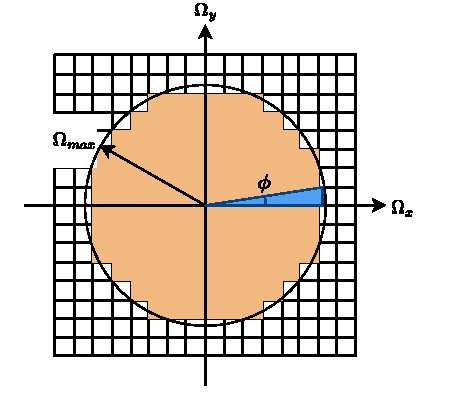
\includegraphics[width=0.6\linewidth]{implementation/resolution limit}
    \caption{Maximum measurable angle at the resolution limit}
    \label{fig:4:resolution_limit}
\end{figure}

Each of the coefficients in Discrete Fourier space is spaced by $\Delta\Omega = \frac{2 \pi}{N} \si{\radian}$ where $N$ is the size of the image. Assuming that we can detect changes that involve 1 coefficient shift in the resolution limit, the finest angle shift we can detect is:

\begin{equation}
    \Delta\Phi = \text{sin}^{-1} \left( \frac{\Delta\Omega}{\Omega_{max}} \right)
\end{equation}

Knowing that $\Omega_{max} = 2 \pi \frac{T_s}{T_{max}}$ where $T_s$ is the pixel size and $T_{max}$ is the resolution limit, the optimal angular sampling rate would be:

\begin{equation}
    \Delta\Phi = 
    \text{sin}^{-1} \left( \frac{\cancel{2 \pi} \frac{1}{N}}{\cancel{2 \pi} \frac{T_s}{T_{max}}} \right) =
    \text{sin}^{-1} \left( \frac{T_{max}}{N T_s} \right)
\end{equation}

In order to avoid repeatedly sampling in the same directions, a random perturbation is added to the projection directions. Empirical results have shown that a value of $\frac{\Delta\Phi}{4}$ offers good results. This value coincides with the average error of the quantisation.

Once the projection parameters are chosen, the volume is projected from quasi-equally spaced angles using the \texttt{xmipp\_angular\_project\_library} program, which was already implemented in Xmipp. This will produce our reference gallery. Prior to this projection, a mask may be applied to the reference volume, so that the alignment is focused on a particular \gls{roi}. 

Additionally, if multiple reference volumes are provided for 3D classification, this step is repeated for each volume. Then all the galleries are combined into a single one, keeping track of the class that each reference image belongs to. in this way, the alignment will not only determine the angular assignment but also the 3D class.

\subsection{Training}
Once a reference gallery is obtained, it will be used to train the vector database used in searches. To do so, \texttt{xmipp\_swiftalign\_train} program is used, which augments the reference gallery by applying random in-plane transformations and uses this augmented dataset to train the FAISS database. 

\subsection{Alignment}
At this point, the previously generated reference gallery and database can be used to align experimental images. This is achieved using \texttt{xmipp\_swiftalign\_query} program. This program will efficiently produce all the in-plane transformations of the reference gallery and then query each of the experimental images in the database. As a consequence, the sampling of the in-plane transformations also needs to be deduced. The rotational sampling estimated for projections still applies for in-plane rotations. Therefore, only the shift sampling rate needs to be computed.

This sampling rate is calculated assuming that for Nyquist a shift of $1 \si{px}$ can be detected. As a consequence, this sampling can be scaled proportionally to the actual resolution limit:

\begin{equation}
    \Delta s = 1 \si{px} \frac{T_{max}}{T_{nyq}} = 1 \si{px} \frac{T_{max}}{2 T_{s}}
\end{equation}

\subsection{Alignment consensus}
We can leverage the speed offered by our alignment method to enhance its outcomes. For this purpose, we can perform multiple alignments to consensuate their outputs, ensuring we retain results that we are confident about. This novel approach enables us to balance speed and accuracy according to the user's requirements. The underlying principle behind the consensus is that we prioritise using fewer particles for reconstruction rather than numerous poorly aligned ones.

Nevertheless, the alignment algorithm is deterministic, meaning that running it multiple times will consistently yield the same results. To overcome this deterministic behaviour, we can generate multiple galleries. As mentioned earlier, each gallery is created with a unique random perturbation. By generating multiple galleries, each with its own distinct random perturbation, we can circumvent the deterministic nature of the algorithm by utilising slightly different galleries for each run.

The aim of the consensus step is to combine the outputs of multiple alignments in such a way that particles that were not aligned properly are discarded. Similarly, particles that coincided in their alignment get their results averaged. An example of such as consensus is displayed in Figure \ref{fig:4:angular_consensus_example}. This figure illustrates that when all alignments produce similar results, there is consensus among them. Contrary to this, if the 3D alignments have disperse results, there is no consensus and the particle should be discarded.

\begin{figure}[htbp]
    \centering
    \begin{subfigure}[b]{0.45\textwidth}
         \centering
         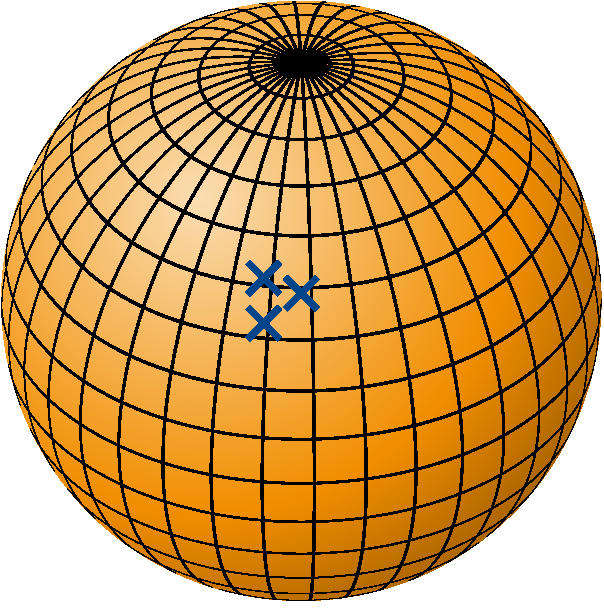
\includegraphics[width=\linewidth]{implementation/consensus/angular consensus 1}
         \caption{Consensus}
    \end{subfigure}
    \hfill
    \begin{subfigure}[b]{0.45\textwidth}
         \centering
         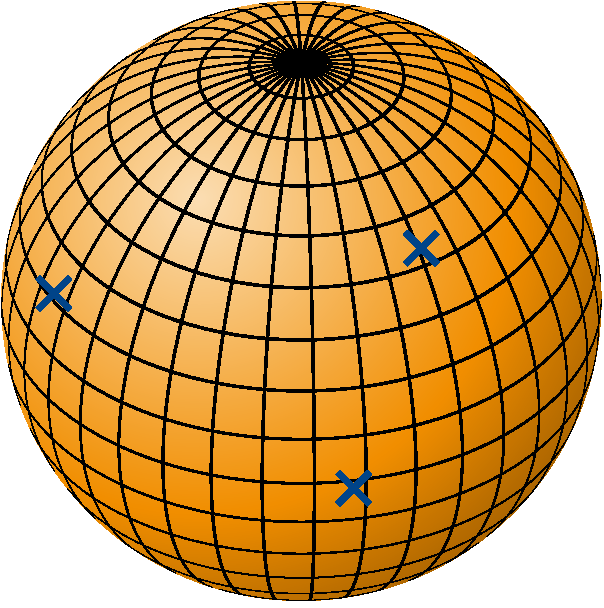
\includegraphics[width=\linewidth]{implementation/consensus/angular consensus 2}
         \caption{No consensus}
    \end{subfigure}
    \caption{Illustration of angular consensus}
    \label{fig:4:angular_consensus_example}
\end{figure}

Note that the previous example was provided with 3 repetitions for consensus. Nevertheless, the implementation is generalised for any number of classifications. Using this principle, we have elaborated a list of criteria to filter particles. If any of the criteria is not met, the particle will be dropped from reconstruction.

\begin{itemize}
    \item The angular assignment is validated by calculating the average angular assignment of the runs. Then, the distance from this average to the samples is computed. The angular assignment is considered to be valid only if more than the $50 \si{\percent}$ of alignments are closer than the angular sampling rate ($\Delta\Phi$). If so, this average angular assignment is used for reconstruction.

    The averaging of angular assignments must be done in quaternion space. Quaternions are an extension to the complex number system which are useful for representing the orientation in 3D space. Contrary to the Euler angles, which are more intuitive, quaternions are not subjected to the gimbal lock issue, making operations easier. In spite of this, the alignment parameters are usually represented with Euler angles. Hence, the Euler angles of the alignment need to be converted to quaternions.

    \begin{equation}
    \begin{split}
    q_0 = 
    \text{cos}\left( \frac{\phi}{2} \right) \cdot \text{cos}\left( \frac{\theta}{2} \right)  \cdot \text{cos}\left( \frac{\psi}{2} \right) -
    \text{sin}\left( \frac{\phi}{2} \right) \cdot \text{sin}\left( \frac{\theta}{2} \right)  \cdot \text{sin}\left( \frac{\psi}{2} \right) \\
    q_1 = 
    \text{cos}\left( \frac{\phi}{2} \right) \cdot \text{cos}\left( \frac{\theta}{2} \right)  \cdot \text{sin}\left( \frac{\psi}{2} \right) +
    \text{sin}\left( \frac{\phi}{2} \right) \cdot \text{sin}\left( \frac{\theta}{2} \right)  \cdot \text{cos}\left( \frac{\psi}{2} \right) \\
    q_2 = 
    \text{cos}\left( \frac{\phi}{2} \right) \cdot \text{sin}\left( \frac{\theta}{2} \right)  \cdot \text{cos}\left( \frac{\psi}{2} \right) -
    \text{sin}\left( \frac{\phi}{2} \right) \cdot \text{cos}\left( \frac{\theta}{2} \right)  \cdot \text{sin}\left( \frac{\psi}{2} \right) \\
    q_3 = 
    \text{sin}\left( \frac{\phi}{2} \right) \cdot \text{cos}\left( \frac{\theta}{2} \right)  \cdot \text{cos}\left( \frac{\psi}{2} \right) +
    \text{cos}\left( \frac{\phi}{2} \right) \cdot \text{sin}\left( \frac{\theta}{2} \right)  \cdot \text{sin}\left( \frac{\psi}{2} \right)
    \end{split}
    \end{equation}

    where $\phi$ is corresponds to the \texttt{rot} parameter, $\theta$ is the \texttt{tilt} parameter and $\psi$ is the in plane rotation.

    The average of quaternions is not trivial either. We have implemented the solution described by \citeauthor{landis2007} in their paper on Quaternion Averaging. This solution uses a \gls{mle} of the average where the average distance from the centroid to the samples is optimised\cite{landis2007}. To do so, the first step is to ensemble a matrix with all the quaternions as rows:

    \begin{equation}
        \bm{Q} = 
        \begin{bmatrix}
            w_1 \bm{q_1}^T \\
            w_2 \bm{q_2}^T \\
            \vdots \\
            w_N \bm{q_N}^T
        \end{bmatrix}
    \end{equation}

    where $w_i$ is the weight associated to each quaternion. For our case, all quaternions will be equally weighted with $w_i = N^{-1}$. Then, the average quaternion can be calculated as the principal eigenvector of $\bm{Q}^T\bm{Q}$.

    Regarding the validation of the average, the quaternion distance is defined as:

    \begin{equation}
        \Delta q = 2 \text{cos}^{-1} \left( \frac{1 - \left\Vert \bm{q_1} - \bm{q_2} \right\Vert^2}{2} \right)
    \end{equation}

    Therefore the criteria to keep a particle is that at least $\frac{N}{2}$ comply with:

    \begin{equation}
        2 \text{cos}^{-1} \left( \frac{1 - \left\Vert \bm{q_i} - \bm{\overline{q}} \right\Vert^2}{2} \right) \leq \Delta\Phi
    \end{equation}
    

    \item Similarly to the previous criteria, the centroid of the shift assignment is computed to validate the shift assignment. $50 \si{\percent}$ or more alignments should be less than the shift sampling rate apart from this centroid. When validated, this centroid is used for reconstruction.

    Formally, the average shift is defined as:

    \begin{equation}
        \overline{\bm{s}} = \frac{1}{N} \sum_{i=1}^{N} \bm{s_i}
    \end{equation}

    Then the alignments agree only if more than $\frac{N}{2}$ alignments comply with:

    \begin{equation}
        \left\Vert \bm{s_i} - \overline{\bm{s}}  \right\Vert \leq \Delta s
    \end{equation}

    \item When a 3D classification is performed, each alignment will vote for a class. If there is no absolute majority, there is no consensus. Otherwise, the mode class is selected (which has been elected by more than the $50 \si{\percent}$ of alignments).
    
\end{itemize}

\subsection{Reconstruction}
At this point the alignment particles are split into two equally sized random subsets. This is done in order to be able to compute the \gls{fsc} between two reconstructions in the next step. Each of these subsets is used to reconstruct a volume using \texttt{xmipp\_reconstruct\_fourier} program (or its \gls{gpu} accelerated variant\cite{strelak2019}), which has been already implemented in Xmipp. As the name of the program suggests, the reconstruction is performed using the Fourier back-projection algorithm, detailed in Chapter \ref{chap:state_of_the_art}. Each of these volumes is known as \textit{half-map}, because they were obtained from half of the particles.

\subsection{Resolution estimation and post processing}
The final step involves comparing both half-maps to determine the resolution of the map. Since particles are aligned independently, each half-map was obtained separately. Consequently, regions that show strong correlation in both maps can be attributed to the signal, while uncorrelated regions are considered as noise.

The correlation between the Fourier coefficients for each frequency is measured using the \gls{fsc} function, which was described in Chapter \ref{chap:state_of_the_art}. This function provides a correlation function in terms of spatial frequency.

Typically, the \gls{fsc} function exhibits a low-pass behaviour. The frequency at which this function crosses a specific threshold (usually $0.5$ or $0.143$) indicates the resolution of the map. This resolution represents the level of detail that can be reliably represented in the volume.

Once the map's resolution is determined, both half-maps are averaged and then subjected to low-pass filtering up to the previously obtained resolution. This filtering step is performed to prevent overfitting caused by noise, as it effectively reduces the number of parameters to be estimated\cite{scheres2012}. The resulting filtered average volume can be used as the reference volume for the next iteration or as the final output volume.

\end{document}
